\textbf{3.} Considere la siguiente gramática:
\begin{eqnarray*}
  S &\rightarrow& aSb\ |\ A\\
  A &\rightarrow& aAd\ |\ cBd\\
  B &\rightarrow& aBb\ | ab
\end{eqnarray*}
Aplica el algoritmo CYK para verificar si las cadenas cabd y aabb se pueden generar con la gramática.
Muestra y explica el proceso de ejecución del algoritmo y si realizas alguna transformación de la gramática
indica el motivo y la técnica usada. \newline

\textbf{Solución.} Primero, llevemos nuestra gramática a la FNC\footnote{Forma Normal de Chomsky.}
\begin{enumerate}
\item Eliminamos producciones unitarias:
\begin{eqnarray*}
S &\rightarrow& aSb\ |\ aAd\ |\ cBd\\
A &\rightarrow& aAd\ |\ cBd\\
B &\rightarrow& aBb\ |\ ab.
\end{eqnarray*}
\item Agregando producciones en FNC:
\begin{eqnarray*}
S &\rightarrow& aSb\ |\ aAd\ |\ cBd\\
A &\rightarrow& aAd\ |\ cBd\\
B &\rightarrow& aBb\ |\ ab\\
A' &\rightarrow& a\\
B' &\rightarrow& b\\
C' &\rightarrow& c\\
D' &\rightarrow& d\\
T_1 &\rightarrow& A'S\\
T_2 &\rightarrow& A'A\\
T_3 &\rightarrow& C'B\\
T_4 &\rightarrow& A'B.
\end{eqnarray*}
\item Sustituyendo en nuestra gramática original tenemos que
\begin{eqnarray*}
S &\rightarrow& T_1B\ |\ T_2D'\ |\ T_3D'\\
A &\rightarrow& T_2D'\ |\ T_3D'\\
B &\rightarrow& T_4D'\ |\ A'B'\\
A' &\rightarrow& a\\
B' &\rightarrow& b\\
C' &\rightarrow& c\\
D' &\rightarrow& d\\
T_1 &\rightarrow& A'S\\
T_2 &\rightarrow& A'A\\
T_3 &\rightarrow& C'B\\
T_4 &\rightarrow& A'B.
\end{eqnarray*}
\end{enumerate}
Ahora que nuestra gramática esta en FNC, podemos aplicar el algoritmo CYK\footnote{Me basaré en el libro: Teoría de autómatas,
lenguajes y computación, de JOHN E. HOPCROFT, RAJEEV MOTWANI, y JEFFREY D. ULLMAN.}:

%\begin{center}
%        \begin{tabular}{| c c c c }
%              S & & & \\
%              $T_3$ & - & & \\
%              - & $B$ & - & \\
%              C' & A' & B' & D' \\ \hline
%              c & a & b & d
%        \end{tabular}
%\end{center}

%\begin{center}
%        \begin{tabular}{| c c c c }
%              B & & & \\
%              $T_4$ & - & & \\
%              - & $B$ & - & \\
%              A' & A' & B' & B' \\ \hline
%              a & a & b & b
%        \end{tabular}
%\end{center}
%cabd.png
\begin{multicols}{2}
Caso cabd:
\begin{center}
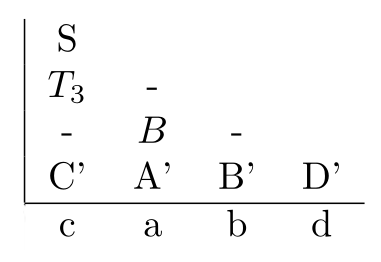
\includegraphics[scale=0.30]{./cabd.png}
\end{center}

Caso aabb:
\begin{center}
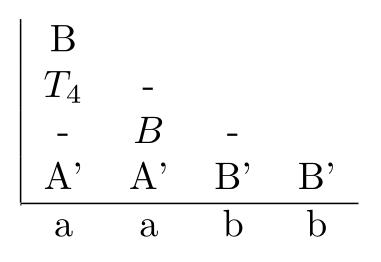
\includegraphics[scale=0.30]{./aabb.png}
\end{center}
\end{multicols}

Como podemos ver, el caso ``cabd'' logra procesar la cadena y por tanto la gramática la genera.
En el caso ``aabb'' no se logra procesar la cadena hasta $S$ y por tanto nuestra gramática no le genera.
